
% On définit le type de document, de papier et la grosseur des caractères.
\documentclass[letterpaper,11pt]{article}

% Trois lignes liées à l'ordinateur avec lequel on produit le document.
\usepackage[utf8]{inputenc}
\usepackage{titling}
\usepackage{amsthm}

% Highlight text
\usepackage{soul} % for the command \hl

% Bibliographie
\usepackage[
backend=biber,
style=alphabetic,
sorting=ynt
]{biblatex}
\addbibresource{Bib1.bib}

\usepackage{dsfont}
\usepackage{layout}
\usepackage{cancel}
\usepackage[french]{babel}
\usepackage[T1]{fontenc}
\usepackage[utf8]{inputenc}
\usepackage[document]{ragged2e}
\usepackage[top=2cm,bottom=2cm,left=2.5cm,right=2.5cm,includehead=true,headheight=1cm]{geometry}%Pour ajustement des marges.
\usepackage{amsbsy}%Accès à des symboles mathématiques
\usepackage{amsfonts}%Accès à des symboles mathématiques
\usepackage{amssymb}%Accès à des symboles mathématiques
\usepackage{bm}%Pour mettre en gras n'importe quel symbole.
\usepackage{enumerate}%Pour les listes d'énumération.
\usepackage{parskip}%Pour pouvoir modifier l'espace entre les paragraphes.
\usepackage{setspace}%Pour pouvoir modifier l'espace entre les lignes.
\usepackage{upgreek}%Pour accéder aux lettres grecques en romain.
\usepackage[b]{esvect}%Permet de créer des vecteurs.
\usepackage{wasysym}
\usepackage{afterpage}
\usepackage{ stmaryrd }
\usepackage{minted}
\usepackage{mathtools}
\usepackage{placeins}
\usepackage{hyperref}
\usepackage{adjustbox}
\usepackage{booktabs}
\usepackage{rotating}
\usepackage{colortbl}
\usepackage{xcolor}


%Symboles fréquents
\newcommand{\N}{\mathbb{N}}
\newcommand{\R}{\mathbb{R}}
\newcommand{\C}{\mathbb{C}}
\newcommand{\I}{\mathbb{I}}
\newcommand{\Z}{\mathbb{Z}}
\newcommand{\Q}{\mathbb{Q}}
\newcommand{\E}{\mathbb{E}}
\newcommand{\?}{\stackrel{?}{=}}
\let\epsilon\varepsilon
\newcommand{\der}{\text{d}}

%Mettre en gras ET italique le paramètre de la fonction
\newcommand{\gras}[1]{\textbf{\textit{#1}}} 

\newcommand\blankpage{%
    \null
    \thispagestyle{empty}%
    \addtocounter{page}{-1}%
    \newpage}%page vierge


\newcommand{\probVar}[1]{\text{Var}\left(#1\right)} %Variance
\newcommand{\probCov}[1]{\text{Cov}\left(#1\right)} %Variance
\newcommand{\probP}[1]{\mathds{P}\left{#1\right}} %P de probabilités
\newcommand{\probE}[1]{\mathbb{E}\left[#1\right]} %E de espérance

\usepackage{hyperref}%'Linker' des équations et sources

%Les quatre lignes qui suivent définissent l'espace entre les paragraphes, l'indentation, l'espace entre les lignes et la distance entre une boite et ce qu'elle contient.
\parskip=10pt 
\parindent=0pt
\onehalfspacing
\fboxsep=9pt

%Parenthèses
\newcommand{\bgl}{\bigl(}
\newcommand{\Bgl}{\Bigl(}
\newcommand{\bggl}{\biggl(}
\newcommand{\Bggl}{\Biggl(}
\newcommand{\bgr}{\bigr)}
\newcommand{\Bgr}{\Bigr)}
\newcommand{\bggr}{\biggr)}
\newcommand{\Bggr}{\Biggr)}

\renewcommand\thesection{\arabic{section}}
\renewcommand\thesubsection{\thesection.\arabic{subsection}}

\begin{document}

\begin{titlepage}
    \centering
    
\includegraphics[width=0.3\textwidth]{udem.png}\par\vspace{1cm} % Replace with your logo file
    {\scshape\LARGE Université de Montréal \par}
    \vspace{1cm}
    {\scshape\Large Département d’Informatique et de Rechercher Opérationnelle\par}
    \vspace{1.5cm}
    {\huge\bfseries Rapport Devoir 3\par}
    \vspace{1.5cm}
    {\Large\itshape Nguyen-Xuan-Bach Bui\par}
    \vfill
    {\Large IFT6512 - Programmation stochastique\par}
\end{titlepage}

All codes are available at \url{https://github.com/BNXBach/Work_stuffs_A2025/tree/main/TP_IFT}

\section*{Les données}

On utilise directement les données de \cite{gurobi} pour les algorithmes. Les 2 fichiers "mu.pkl" et "sigma.pkl" contiennent les rendements $\mu$ et la matrice de covariance $\Sigma$. Le site Gurobi a appliqué la technique de contraction (shrinkage) pour minimiser l'effet sur les algorithmes qui vient de l'incertitude et la sensibilité des données.

Pour lire les fichiers .pkl qui sont d'origine de Python, on utilise le package Pandas de Julia qui a la fonction read\_pickle. Il y a aussi d'autres options avec PyCall qui sont plus effcicaces mais on a trouvé que Pandas était la solution la plus simple. 

\section*{Les portefeuilles}
On utilise Gurobi pour tous les portefeuille. La structure des résultats de chaque portefeuille est:
\begin{itemize}
    \item La structure du solveur du portefeuille
    \item Les positions les plus grandes du portefeuille optimisé
    \item Les critères comme le rendement, la variance, etc...
\end{itemize}

Chaque portefeuille a ses propres hyperparamètres. Alors, pour mieux comparer les portefeuilles, on a essayé de choisr ces hyperparamètres pour faire correspondre le rendement de ces portefeuilles à celui du portefeuille uniforme. On veut observer s'il y a un portefeuille qui est clairement mieux que le reste ou s'ils sont les mêmes et expliquer pourquoi.

Dans ce rapport, on a décidé de ne pas autoriser les transactions à découvert (short selling) afin de comparer notre code Julia avec celui en Python de \cite{gurobi}. De plus, si on permet ces transactions, le portefeuille uniforme ne peut pas l'utiliser alors les comparaisons seront un peu moins correctes.

Par contre, dans le notebook, il y a l'option de faire des transactions à découverte en changeant le paramètre "short\_amount". On a inclu une partie Extra qui parle des portefeuilles avec ces transactions à la fin du rapport. 

\newpage
\section*{Les résultats}
\subsection*{Portefeuille uniforme}
Le portefeuille de base. Les positions sont égaux pour tous les actifs et la somme est 1.

\begin{figure}[H]
    \centering
    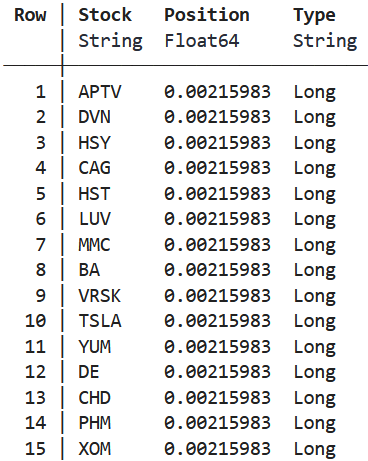
\includegraphics[width=0.4\columnwidth]{unif.png}
    \caption{Position du portefeuille uniforme}
\end{figure}
\FloatBarrier

\begin{table}[htbp]
\centering
\begin{adjustbox}{width=0.55\textwidth,center=\textwidth}
\begin{tabular}{ l c }
\toprule
\textbf{Critère} & \textbf{Valeur}  \\
\midrule
\rowcolor{black!10}Rendement & 0.2328122589140964  \\
Probabilité de perte & 0.458253  \\
\rowcolor{black!10}Perte espérée & -1.6682528134548156  \\
Variance & 4.803074590438797  \\
\bottomrule
\end{tabular}
\end{adjustbox}
\caption{Table de critère: Portefeuille uniforme}
\label{tab:uni}
\end{table}

Avec les autres portefeuilles, on veut le même rendement de celui ici mais avec les autres critères plus petits.

\newpage 
\subsection*{Portefeuille maximisant le rendement}
L'optimisateur est très simple, on garde les contraintes de bases dans \cite{web} et on maximise le rendement $\mu^Tp$ où $p$ est le vecteur de positions des actifs. Il faut noter que ce portefeuille n'est pas un portefeuille Markowitz car il n'y a pas de contrainte sur la variance.


\begin{figure}[H]
    \centering
    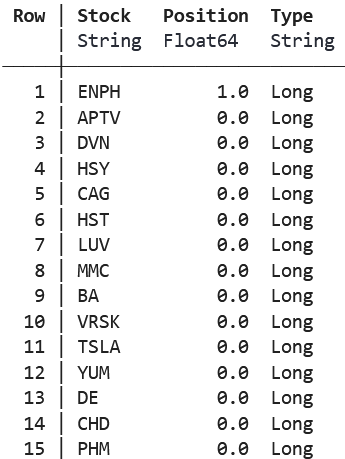
\includegraphics[width=0.4\columnwidth]{maxret.png}
    \caption{Position du portefeuille maximisant le rendement}
\end{figure}
\FloatBarrier

\begin{table}[htbp]
\centering
\begin{adjustbox}{width=0.55\textwidth,center=\textwidth}
\begin{tabular}{ l c }
\toprule
\textbf{Critère} & \textbf{Valeur}  \\
\midrule
\rowcolor{black!10}Rendement & 0.5957955115760344  \\
Probabilité de perte & 0.4782215  \\
\rowcolor{black!10}Perte espérée & -8.462982016430146  \\
Variance & 117.99735282302423  \\
\bottomrule
\end{tabular}
\end{adjustbox}
\caption{Table de critère: Portefeuille maximisant le rendement}
\label{tab:maxreturn}
\end{table}

Un cas extrême juste pour montrer le rendement maximum ce qui est proche de $0.6$. On note que la probabilité de perte n'est pas très loin de celle du portefeuille uniforme. Par contre, la perte espérée est très grande à cause de la variance de l'actif "ENPH" qui est presque 118. 

\newpage 
\subsection*{Portefeuille minimisant la variance}

Le première portefeuille de Markowitz. On garde les contraintes de bases. Puis on ajoute la contrainte sur le rendement attendu $\mu^Tp \geq \bar{\mu}$. L'objectif est de minimiser la variance $p(1,..,n-1)^T\Sigma p(1,...,n-1)$. La raison de prendre seulement $p(1,...,n-1)$ est parce que la dernière position est l'actif sans risque. 

\begin{figure}[H]
    \centering
    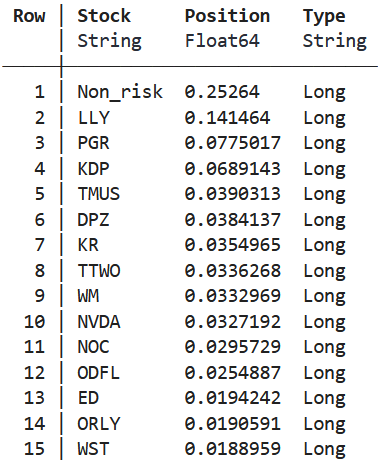
\includegraphics[width=0.4\columnwidth]{minvar.png}
    \caption{Position du portefeuille minimisant la variance}
\end{figure}
\FloatBarrier

\begin{table}[htbp]
\centering
\begin{adjustbox}{width=0.55\textwidth,center=\textwidth}
\begin{tabular}{ l c }
\toprule
\textbf{Critère} & \textbf{Valeur}  \\
\midrule
\rowcolor{black!10}Rendement & 0.2328122589146225  \\
Probabilité de perte & 0.425473  \\
\rowcolor{black!10}Perte espérée & -0.9041005541959475  \\
Variance & 1.5193125909069476  \\
\bottomrule
\end{tabular}
\end{adjustbox}
\caption{Table de critère: Portefeuille minimisant la variance}
\label{tab:minvar}
\end{table}

On retrouve le même rendement que celui du portefeuille uniforme mais cette fois-ci, on a une probabilité de perte plus petite (3\% moins) et aussi une variance significativement plus basse ($1.51$ vs $4.8$). C'est un portefeuille plus efficient et donc on veut vérifier si les autres portefeuilles peuvent surpasser celui-ci.

\newpage 
\subsection*{Portefeuille minimisant la risque de perte}
L'optimisateur est exactement le même de celui dans \cite{web}. Pour le niveau de $\alpha$, on l'a choisi pour faire correspondre à celui du portefeuille minimisant la variance et on voulais observer si le rendement est plus grand ou la variance est plus basse de manière significative. 

\begin{figure}[H]
    \centering
    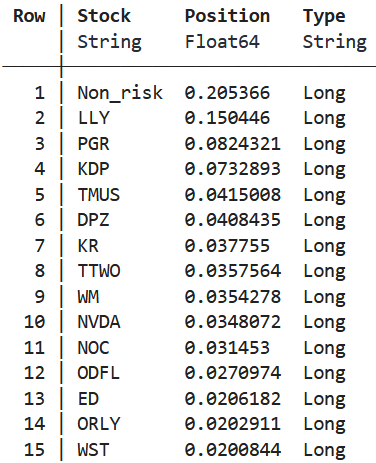
\includegraphics[width=0.4\columnwidth]{minrisk.png}
    \caption{Position du portefeuille minimisant la risque de perte}
\end{figure}
\FloatBarrier


\begin{table}[htbp]
\centering
\begin{adjustbox}{width=0.55\textwidth,center=\textwidth}
\begin{tabular}{ l c }
\toprule
\textbf{Critère} & \textbf{Valeur}  \\
\midrule
\rowcolor{black!10}Rendement & 0.24629656407029377  \\
Probabilité de perte & 0.4258305  \\
\rowcolor{black!10}Perte espérée & -0.9618467183420845  \\
Variance & 1.7179471815895253  \\
\bottomrule
\end{tabular}
\end{adjustbox}
\caption{Table de critère: Portefeuille minimisant la risque de perte}
\label{tab:minrisk}
\end{table}

On a obtenu un portefeuille presque identitique au portefeuille minimisant la variance. La position de l'actif sans risque est plus petit mais sauf cette différence, les autres actifs sont les mêmes et leurs positions sont similaires aussi. De même pour les critères, on voit un rendement légèrement plus grand mais aussi une variance plus élevée. Pour la probabilité de perte et la perte espérée, il n'y a pas de grande différence entre les 2. 

Pour éliminer des bruits, on a relancé notre code plusieurs fois et la conclusion est toujours la même, les 2 portefeuilles peuvent être considérés comme identique et la différence vient des bruits/simulations. 


\newpage 
\subsection*{Portefeuille maximisant l'utilité}
Un autre portefeuille de Markowitz mais on n'optimise pas exactement une critère de comparaison. Il y a juste un hyperparamètre $\gamma$ et l'objectif est de maximiser l'utilité $\mu^Tp -\dfrac{\gamma}{2}p^T\Sigma p$. Ici, on a essayé de faire tuner $\gamma$ pour faire correspondre la probabilité de perte à celle du portefeuille minimisant cette quantité.

\begin{figure}[H]
    \centering
    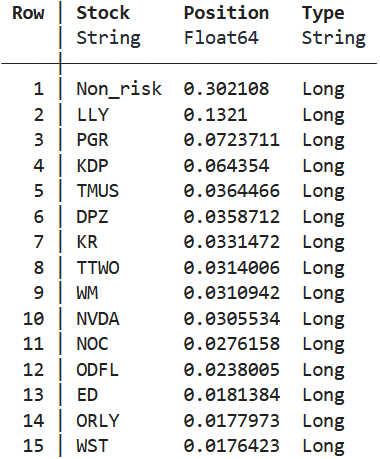
\includegraphics[width=0.4\columnwidth]{maxutil.png}
    \caption{Position du portefeuille maximisant l'utilité}
\end{figure}
\FloatBarrier

\begin{table}[htbp]
\centering
\begin{adjustbox}{width=0.55\textwidth,center=\textwidth}
\begin{tabular}{ l c }
\toprule
\textbf{Critère} & \textbf{Valeur}  \\
\midrule
\rowcolor{black!10}Rendement & 0.2187260979991341  \\
Probabilité de perte & 0.425025  \\
\rowcolor{black!10}Perte espérée & -0.8438230721495293  \\
Variance & 1.324840719543774  \\
\bottomrule
\end{tabular}
\end{adjustbox}
\caption{Table de critère: Portefeuille maximisant l'utilité}
\label{tab:maxutil}
\end{table}

On peut voir que c'est aussi un portefeuille similaire que les autres parce que les top actifs sont encore les mêmes.

On compare plus en détail ici. On note qu'une petite modification de la probabilité de perte entraîne une grande modification du rendement/variance. C'est pourquoi ces 3 portefeuilles sont différents. La chose importante à noter ici est que les critères changent de même façon entre les portefeuilles. Il n'y a rien d'inhabituel et le taux de changement est le même. Même si ces portefeuilles sont différents, leurs efficacité sont identiques.

\newpage 
\subsection*{Portefeuille minimisant la variance avec diversification}

L'objectif de ce portefeuille est le même que le portefeuille minimisant la variance. On ajoute une contrainte de nombre d'investissments $K=35$. Pour le faire, on crée 2 bornes pour des positions, une borne maximum $u$ surtout pour limiter l'actif sans risque et une borne minimum $l$ pour que les positions aient plus de poids si on décide de l'investir dedans. On a choisi $u = 0.1$ et $l=0.01$ alors il faut que des positions soient $1\%$ au minimal et $10\%$ au maximal. Puis, on ajoute une variable binaire $b$ comme décision d'investir. Finalement, la contrainte $\sum b_i\geq K$ va forcer la diversification et la contrainte $p_i\geq l*b_i$ et $p_i \leq b_i$ vont forcer les positions.

\begin{figure}[H]
    \centering
    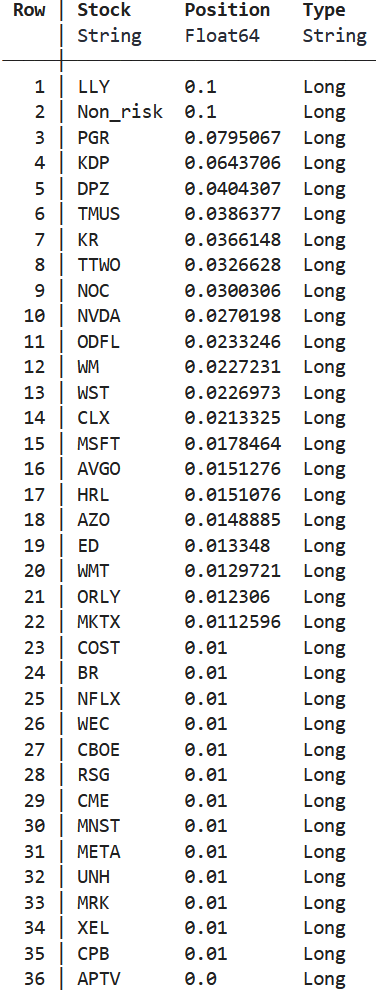
\includegraphics[width=0.362\columnwidth]{div.png}
    \caption{Position du portefeuille minimisant la variance avec diversification}
\end{figure}
\FloatBarrier

\begin{table}[htbp]
\centering
\begin{adjustbox}{width=0.55\textwidth,center=\textwidth}
\begin{tabular}{ l c }
\toprule
\textbf{Critère} & \textbf{Valeur}  \\
\midrule
\rowcolor{black!10}Rendement & 0.23281225891409638  \\
Probabilité de perte & 0.426822  \\
\rowcolor{black!10}Perte espérée & -0.9217981649353686  \\
Variance & 1.5746040856327332  \\
\bottomrule
\end{tabular}
\end{adjustbox}
\caption{Table de critère: Portefeuille minimisant la variance avec diversification}
\label{tab:div}
\end{table}
\FloatBarrier

Évidemment, le portefeuille est différent d'un portefeuille Markowitz. C'est intéressant de voir que l'actif "LLY" est maximisé (son rendement est $0.33$ et sa variance est $8.71$). Si on le compare avec le portefeuille minimisant la variance, on peut noter que le rendement est le même mais la variance est plus grande. Alors, ce portefeuille est moins efficace mais c'est légère et on peut le négliger. Le but de ce portefeuille est de limiter la stratégie d'investir le plus possible dans l'actif sans risque pour miniser la variance/risque et nous forcer à chercher d'autre part. Ce n'est pas le portefeuille le plus efficace mais c'est possible que c'est le seul portefeuille réalisable s'il y a des restrictions sur l'actif sans risque. 

\newpage 
\section*{Conclusion}

\begin{figure}[H]
    \centering
    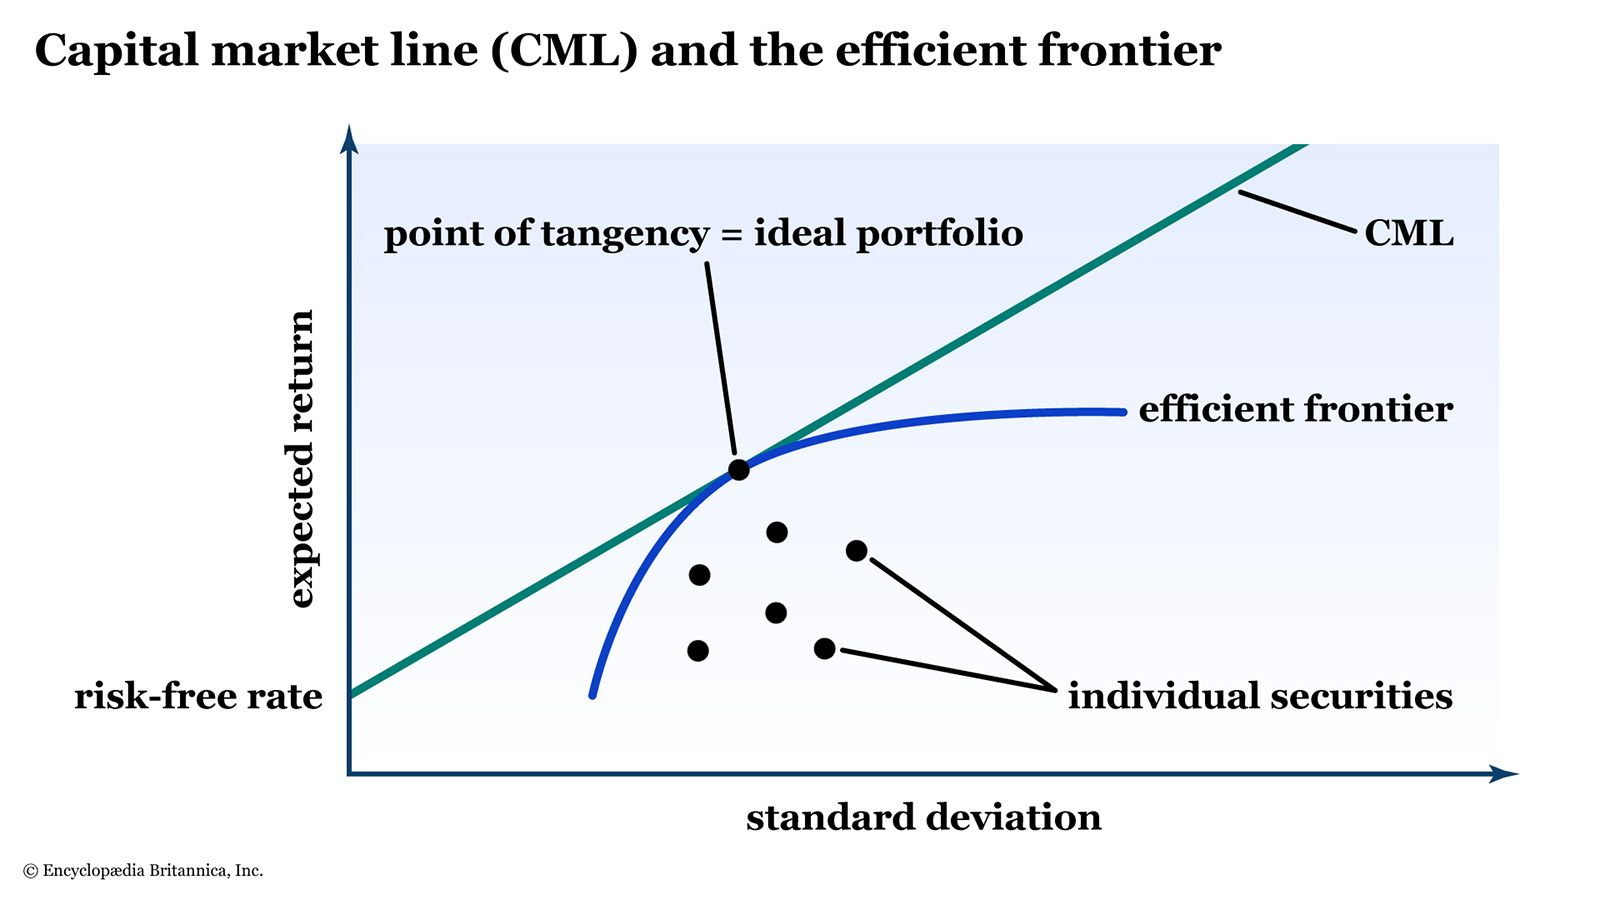
\includegraphics[width=0.7\columnwidth]{mpt.jpg}
    \caption{Modern Portfolio Theory}
\end{figure}
\FloatBarrier

On a 2 résultats principales ici:
\begin{enumerate}
    \item Le portefeuille minimisant la probabilité de perte est aussi un portefeuille Markowitz. C'est-à-dire il reste sur la frontière efficace comme dans la Figure 7 [\cite{web2}]. Il n'y a pas un meilleur portefeuille parce qu'ils sont tous efficaces alors cela dépend de l'investisseur. Ce que le portefeuille minisant la probabilité de perte introduit est un autre paramètre pour l'agent.
    Au lieu de choisir un rendement ou une variance idéale, un agent averse au risque peut juste simplement indiquer sa tolérance pour le risque et il peut trouver un portefeuille efficace. \newline
    \item Forcer la diversification n'a pas un impact très grand sur l'efficacité du portefeuille. Dans des cas où la diversification est nécessaire, on peut le faire sans perdre trop de l'argent. De plus, on peut éviter aussi des cas extrêmes comme un actif qui perd tout soudainment par exemple. On peut penser la diversification comme un étape extra pour minimiser le risque.
\end{enumerate}

\newpage 
\section*{Extra: Short-selling}
On veut juste montrer ici l'effet des transactions à découvert sur le portefeuille minimisant la variance. On a testé et on a arrivé à la même conclusion en haut. On a limité le poids d'une telle transaction à $-0.1$ comme dans le cours.

\begin{figure}[H]
    \centering
    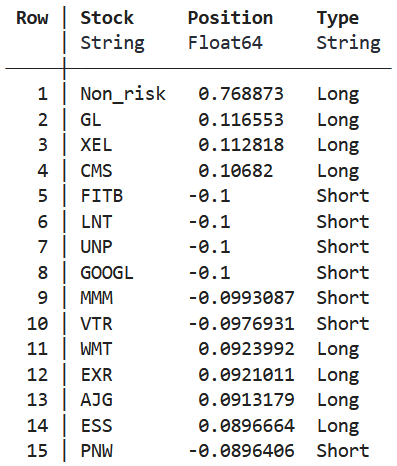
\includegraphics[width=0.4\columnwidth]{short.png}
    \caption{Position du portefeuille minimisant la variance avec short-selling}
\end{figure}
\FloatBarrier

\begin{table}[htbp]
\centering
\begin{adjustbox}{width=0.55\textwidth,center=\textwidth}
\begin{tabular}{ l c }
\toprule
\textbf{Critère} & \textbf{Valeur}  \\
\midrule
\rowcolor{black!10}Rendement & 0.23281225913593068  \\
Probabilité de perte & 0.171026  \\
\rowcolor{black!10}Perte espérée & -0.1312484409296736  \\
Variance & 0.06010323283269285  \\
\bottomrule
\end{tabular}
\end{adjustbox}
\caption{Table de critère: Portefeuille minimisant la variance avec short-selling}
\label{tab:div}
\end{table}
\FloatBarrier

On peut voir que la variance est vachement plus basse que si on n'autorise pas de short-selling. En gros, la stratégie reste le même, c-à-d optimiser pour acheter le plus possible l'actif sans risque.
Donc, le short-selling est un outil très fort et pertinent pour augmenter l'efficacité des portefeuilles.

\newpage
\section*{Références + Utilisation de l'intelligence artificielle}

\printbibliography

\subsection*{Utilisation de l'intelligence artificielle}
J'ai utilisé l'IA pour:
\begin{itemize}
    \item Aide avec des syntaxes de Latex pour écrire ce rapport.
    \item Aide avec des syntaxes de Julia pour construire des dataframes pour la visualisation.
\end{itemize}
Le contenu de ce rapport est écrit sans utilisation de l'IA. La partie code Julia + les algorithmes sont basés sur \cite{gurobi} et \cite{web}
\end{document}




